\chapter{Application -- Theoretical Background and Practical Implementation}
%\section{Theoretical background}

\section{Geometric Brownian Motion}
    \textit{Geometric Brownian Motion} is frequently used as a model for simulating diverse variables such as financial processes (for example stock price). In order to well define what a \textit{GBM} is, it essential to first describe several terms that will help further understanding.
    
    \subsection{Random Walk}
        In mathematics \textit{Random Walk} is an example of a stochastic process that illustrates how objects might travel if they are randomly-moving, see more detail here \cite{randomWalk}.
        
        If 1-dimensional space is considered, then it is best to present the action on the number line.
        \begin{figure}[H]
            \centering
            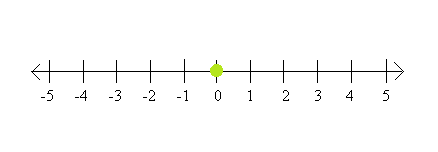
\includegraphics{img/numberLine.png}
            \caption{Number line with starting point $P_0=0$}
            \caption*{$P$ stands for \textit{Position}.}
            \label{fig:numberLine_start}
        \end{figure}
        
        Random walk starts at the point 0 (fig. \ref{fig:numberLine_start}). Then there occur $N$ steps, $N \in \mathbb{N}_+$, and each of them is likely to move to the right ($+1$) or to the left ($-1$) by 50\%. Example outcome after 4 steps could be as follows:
        
        \begin{figure}[H]
            \centering
            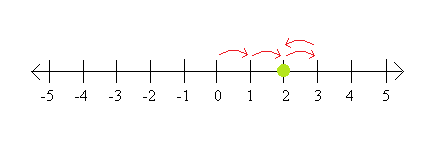
\includegraphics{img/numberLine_end.png}
            \caption{Sample outcome for $N=4$.}
            \label{fig:numberLine_end}
        \end{figure}
        
        In this example steps could be described as $a_1 = a_2 = a_3 = 1$ and $a_4 = -1$, meaning first 3 steps were to the right, while the last one was to the left. The outcome (position of the green dot after all steps) is $P_4 = 2$ (fig. \ref{fig:numberLine_end}).
        
        Therefore, the position of the green dot can specified by the following formula:
        \[  % \ldots looks better than ...
        P_N = a_1 + a_2 + a_3 + \ldots + a_N
        \]
        
        \textit{Random Walk} $RW$ can then defined as the following series:
        \[
        RW = \{P_n, n \in N\}
        \]
        %
        Since each move has the same probability to be $-1$ or $1$ then the expected value of such series (final position of the dot) can be easily calculated:
        \[
        \mathbb{E}(RW) = 0
        \]
        
        An interesting observation can be made when calculating estimated value of a series that is the same as \textit{Random Walk} but its values are squares of original values.
        % I should use \(...\) instead of $...$
        Then:
        \[
        \mathbb{E}({RW}^2) = \sum_{i=1}^{N} a_{i} + 2*\sum_{1 \leq i \leq j \leq N}^{N} a_{i}*a_{j} = N
        \]
        
        Therefore, the average distance, that the dot will appear on at the end of the walk will be at \(\sqrt{N}\) blocks from the starting position.
        
    \subsection{Wiener Process}
        \textit{Wiener Process} is also usually called \textit{Standard Brownian Motion}. It is a continuous-time stochastic process named after Norbert Wiener for his work on 1D \textit{Brownian Motion}.
        %
        \textit{Wiener Process}, as well as \textit{Random Walk}, starts at 0 (\( W(0) = 0 \)) and its increment follows Gaussian distribution with mean \(0\) and variance \(t-s\) for any \(0\leq s < t \) (more info here \cite{wienerProcess}).
        %
        This way a \textit{Brownian Motion} is basically a \textit{Random Walk} with steps which sizes are random.
        
\section{Options}
    Options are some of the most popular derivative financial instruments. Derivative means in this example that it's value is reliant upon an underlying asset. The most important thing about options, one that distinguishes them from other derivative instruments it the \textbf{optionality} -- contract can, be is not obligatory to be made.
    
    There are 2 main types of options:
    \begin{itemize}
        \item \textbf{Call option} -- the buyer of the call option earns a right (not an obligation) to exercise his option to buy a particular asset from the call option seller for a stipulated period of time.
        \item \textbf{Put option} -- the buyer of the put option earns a right to exercise his option to sell a particular asset to the put option seller for a stipulated period of time ( see definition there \cite{Call_Put_Option_Definition}).
    \end{itemize}
    
    There are several parameters that describe an option, most important ones are:
    \begin{itemize}
        \item \textbf{Expiration Date} -- Specific moment in time by which the holder of the option has to decide whether he wants to exercise (use) the option.
        \item \textbf{Strike Price} -- agreed price at which the derivative underlying asset can be bought or sold (depends on a type of option) when it is exercised.
    \end{itemize}
    
    Further division into option types depends on when the option can be exercised. The most basic one is \textbf{European}-style option -- decision whether option will or will not be exercised is made at the time of option's expiry. Continuous option type is an \textbf{American} option -- option can be exercised at any time before the expiry. Combination of those two can be found in \textbf{Burmudan} Option -- contract can be exercised at specific days before the expiration. In this paper European Options will be presented (more about option types here \cite{Option_Types}).

\section{Black-Scholes Model}
    The Black--Scholes (or also called Black--Scholes--Merton) formula was created back in 1970s by 3 major economists: Fischer Black, Myron Scholes and Robert Merton (Scholes and Merton were awarded Nobel prize for economics in 1997. Certainly same would happen for Black if sadly it was not for his death in 1975).
    
    Their model was a significant breakthrough in world of mathematical models used for pricing derivative instruments. It provides a framework for European-style option valuations, such as calls and puts.
    
    This thesis' aim was not to goo deep into understanding the mathematical background behind the model but rather implement the model in a practical tool that one would be able to effectively use. Therefore more information and specifics can be found either in the original publication \cite{10.2307/1831029} of the model from 1973 in \textit{The Pricing of Options and Corporate Liabilities} of the Journal of Political Economy by Fischer Black and Myron Scholes.
    
    Main formula of the model used for option pricing is as follows:
    \[
    C = S_0\phi(d_1) - Ke^{-rT}\phi(d_2)
    \]
    \[
    P = -S_0\phi(-d_1) + Ke^{-rT}\phi(-d_2)
    \]
    \[
    d_1 = ln\frac{S_0}{K} + (r+\frac{\sigma^2}{2})t
    \]
    \[
    d_2 = d_1 - \sigma\sqrt{t},
    \]
    where:
    \begin{itemize}
        \item $C$ - call option price,
        \item $P$ - put option price,
        \item $S_0$ - underlying asset price at the time being,
        \item $\phi()$ - standardized cumulative normal distribution,
        \item $K$ - strike price,
        \item $r$ - risk free rate (1\% represented as 0.01),
        \item $t$ - time to maturity in years (18 months represented as 1.5),
        \item $\sigma$ - volatility (20\% represented as 0.2).
    \end{itemize}
    
    The formula assumes that the price history of an underlying asset (in this example - a stock price) has a lognormal distribution and follows geometric Brownian motion with constant drift and volatility. 
    \todo{diff eq thats at the core of the model as curiosity}